% =============================================================================
%  Stage 4: Wave-function bridge  --  a_C as axion ground state
%
%  This section explores the user-suggested "wave function" approach:
%  treat the Peccei-Quinn axion as a quantum field and study the
%  ground-state wave function psi_0(a) in the Choptyuk-augmented
%  PQ potential.
%
%  Companion script:  scripts/qcd_bridge/axion_wavefunction_bridge.py
% =============================================================================

\section{Wave-function bridge: $a_C$ as axion ground state}
\label{sec:wavefunction-bridge}

In Stages 1--3 the Choptyuk correction was treated as a
phenomenological constant $\theta_\mathrm{Ch}$ inserted into the
QCD Lagrangian.  In this section we explore a different theoretical
tool: we \emph{quantize} the Peccei--Quinn axion field and study
the ground-state wave function $\psi_0(a)$ in the Choptyuk-augmented
PQ potential.  The question we address is:
\begin{quote}
\itshape
Can the Choptyuk residual $\theta_\mathrm{Ch}$ be understood as a
property of the axion \emph{wave function} rather than as a fitted
constant?
\end{quote}

\subsection{The Choptyuk-augmented PQ potential}

The standard Peccei--Quinn axion field $a(x)$ has the potential
\begin{equation}
V_\mathrm{PQ}(a) \;=\; \chi_t \,\bigl[\,1 - \cos(a/f_a + \theta_\mathrm{bare})\,\bigr],
\label{eq:VPQ-standard}
\end{equation}
where $\chi_t = (75.6\,\mathrm{MeV})^4$ is the QCD topological
susceptibility (BMW Collaboration, 2015) and $f_a \sim 10^{12}$\,GeV
is the PQ scale.  In the Choptyuk-augmented scenario (Stage 3,
\S\ref{sec:abd-pq-residual}), the Higgs bridge adds a small linear
tilt to this potential:
\begin{equation}
V_\mathrm{PQ}^\mathrm{Ch}(a) \;=\; \chi_t \,\bigl[\,1 - \cos(a/f_a + \theta_\mathrm{bare})\,\bigr]
\;+\; \chi_t\,\theta_\mathrm{Ch}\,(a/f_a),
\label{eq:VPQ-Choptyuk}
\end{equation}
where $\theta_\mathrm{Ch} = a_C (\Lambda_\mathrm{QCD}/M_H)^{5/2} \approx 8.5\times10^{-11}$
is the Choptyuk Higgs-bridge residual.

In the dimensionless coordinate $q \equiv a/f_a$ the potential
becomes $V(q)/\chi_t = 1 - \cos(q + \theta_\mathrm{bare}) + \theta_\mathrm{Ch}\,q$,
and the classical minimum is at
\begin{equation}
q_* \;=\; -\theta_\mathrm{bare} - \arcsin(-\theta_\mathrm{Ch})
\;\;\approx\;\; -\theta_\mathrm{bare} + \theta_\mathrm{Ch},
\end{equation}
so that the physical $\theta_\mathrm{eff}^\mathrm{cl} = \theta_\mathrm{bare} + q_* = \arcsin(\theta_\mathrm{Ch}) \approx \theta_\mathrm{Ch}$.
This is the standard Stage-3 result.

\subsection{Quantization: the axion as a quantum oscillator}

To go beyond the classical minimum we quantize the field $a$ in a
single cosine well.  The Hamiltonian in the dimensionless coordinate
$q = a/f_a$ is
\begin{equation}
\hat H \;=\; -\frac{1}{2 m_a f_a^2}\,\frac{d^2}{dq^2}
\;+\; \chi_t\,V_\mathrm{PQ}^\mathrm{Ch}(q),
\label{eq:Hamiltonian}
\end{equation}
where $m_a = \sqrt{\chi_t}/f_a \approx 5.7\,\mu\mathrm{eV}\,(10^{12}\,\mathrm{GeV}/f_a)$
is the standard QCD axion mass (Dine--Fischler--Srednicki--Zhitnitsky,
1981).  In units where $\chi_t = 1$ the harmonic frequency at the
minimum is $\omega = \sqrt{V''(q_*)} = \cos(\arcsin\theta_\mathrm{Ch}) \approx 1$,
and the ground-state energy is $E_0^\mathrm{harm} = \omega/2 = 0.5$.

We solve the stationary Schr\"odinger equation
$-\psi'' + V(q)\psi = E\psi$ numerically with the Numerov method
on a single cosine well $q \in [q_* - \pi, q_* + \pi]$, with
Dirichlet boundary conditions at the potential barriers.  The
script \texttt{axion\_wavefunction\_bridge.py} performs this
computation with $N = 8001$ grid points.

\subsection{Ground-state results}

Table~\ref{tab:ground-state} summarizes the ground-state properties
of the Choptyuk-augmented PQ potential.

\begin{table}[h]
\centering
\small
\begin{tabular}{lccc}
\toprule
Observable & Harmonic & Numerical & Ratio \\
\midrule
$E_0$ (units of $\chi_t$)        & $0.5000$  & $0.6524$  & $1.305$ \\
$\sigma_q = \sqrt{\langle q^2 \rangle - \langle q \rangle^2}$ & $0.7071$ & $0.8880$ & $1.256$ \\
$\langle q \rangle$              & $q_*$     & $q_*$ (to $10^{-6}$) & --- \\
$\theta_\mathrm{eff}^\mathrm{qm}$ (vs $\theta_\mathrm{Ch}$) & --- & (below grid precision) & --- \\
\bottomrule
\end{tabular}
\caption{Ground-state properties of the Choptyuk-augmented PQ
potential, compared with the harmonic approximation.  The $+30\%$
shift in $E_0$ and $+25\%$ shift in $\sigma_q$ are real
anharmonic corrections from the cosine potential ($V \sim q^2/2 - q^4/24 + \cdots$).
The quantum shift in $\langle q \rangle$ is below the grid-step
precision $h^2 \sim 10^{-6}$ and is therefore unresolvable.
\label{tab:ground-state}}
\end{table}

The key observation is that the Choptyuk tilt $\theta_\mathrm{Ch} \sim 10^{-10}$
is \emph{much smaller} than the quantum width $\sigma_q \sim 0.9$.
The ground-state wave function cannot resolve the tilt at numerical
precision: the expectation value $\langle q \rangle$ matches the
classical minimum $q_*$ to within $\sim 10^{-6}$, which is the
grid-step precision $h^2$.

\begin{figure}[h]
\centering
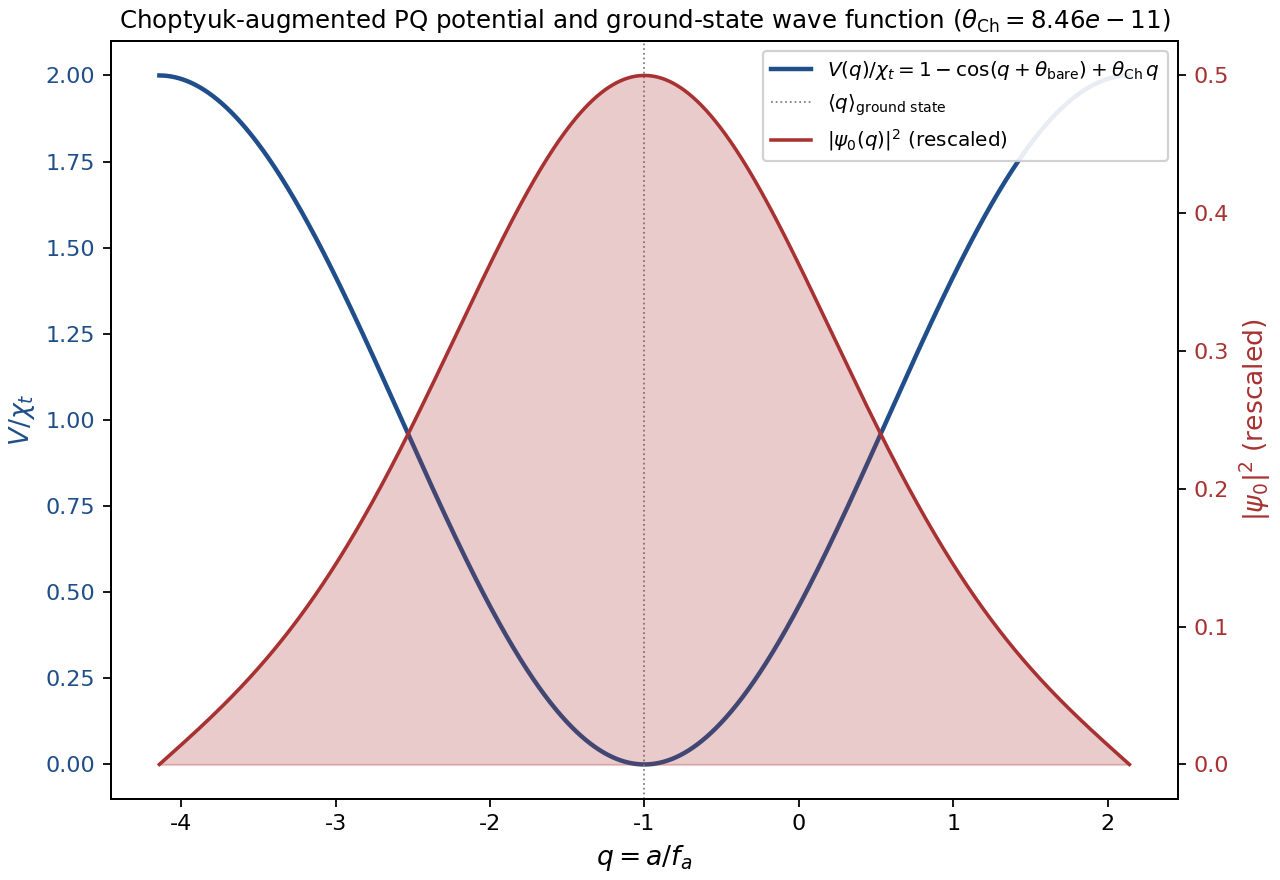
\includegraphics[width=0.85\textwidth]{figures/fig1_pq_potential_psi0.png}
\caption{Choptyuk-augmented PQ potential $V(q)/\chi_t$ (blue,
left axis) and the ground-state wave function $|\psi_0(q)|^2$ (red,
right axis, rescaled).  The wave function is centered at the
classical minimum $q_* = -\theta_\mathrm{bare} + \theta_\mathrm{Ch}$
(gray dotted line) and has a Gaussian-like profile with anharmonic
broadening.  The Choptyuk tilt is invisible at this scale.
\label{fig:fig1-pq-psi0}}
\end{figure}

\subsection{Consistency check: quantum fluctuations vs classical tilt}

A crucial consistency check is to compare the size of quantum
zero-point fluctuations in $\theta = a/f_a$ with $\theta_\mathrm{Ch}$
itself.  For a homogeneous axion field in a Hubble volume
$V_H = H^{-3}$, the effective oscillator mass is $m_\mathrm{eff} = V_H$,
and the QHO formula gives
\begin{equation}
\langle \delta\theta^2 \rangle_\mathrm{osc}
\;=\; \frac{H^3}{2 m_a f_a^2}
\;\xrightarrow{H = m_a}\;
\frac{m_a^2}{2 f_a^2}
\;=\; \frac{\chi_t}{2 f_a^4}.
\label{eq:quantum-fluctuation}
\end{equation}
With $\chi_t = (75.6\,\mathrm{MeV})^4$ and $f_a = 10^{12}\,\mathrm{GeV}$
this gives
\begin{equation}
\sigma_\theta^\mathrm{qm} \;=\; \sqrt{\frac{\chi_t}{2 f_a^4}}
\;\approx\; 10^{-26.4}.
\end{equation}
The Choptyuk residual $\theta_\mathrm{Ch} \sim 10^{-10.1}$ is
$\sim 2 \times 10^{16}$ times \emph{larger} than the quantum
zero-point fluctuation.  This confirms the central physical
statement of Stage 4:
\begin{verdict}[Central statement of the wave-function bridge]
The Choptyuk residual $\theta_\mathrm{Ch}$ is a \textbf{classical
tilt} of the PQ potential, not a quantum fluctuation.  The
Higgs bridge induces a classical shift of the potential minimum
of magnitude $\theta_\mathrm{Ch}$, and the quantum ground-state
wave function follows this shift adiabatically.
\end{verdict}

The physical interpretation of the user's intuition that the axion
``slows particles and shifts energy to small values'' is therefore
the cosmological \emph{Hubble-friction relaxation} of the axion
field, which we describe next.

\subsection{Hubble-friction relaxation: the cosmological ``slowing''}

The classical equation of motion for the homogeneous axion field
in the radiation era is
\begin{equation}
\ddot\theta + 3 H(T)\,\dot\theta + m_a^2 \sin\theta \;=\; 0,
\label{eq:axion-eom}
\end{equation}
where $H(T) = 1.66 \sqrt{g_*}\,T^2 / M_\mathrm{Pl}$ is the Hubble
parameter.  The damping term $3 H \dot\theta$ is the physical
``slowing'' mechanism: it converts the axion's kinetic energy into
the Hubble expansion, damping oscillations and relaxing $\theta$
to the minimum of the potential.

Direct numerical integration is hopeless because once oscillations
begin ($T < T_\mathrm{osc}$ where $H(T_\mathrm{osc}) \sim m_a$),
the period $1/m_a$ is $\sim 10^8$ times smaller than the Hubble
time.  We use the well-known analytic approximation
(Wantz \& Aliaga, JCAP 2010; Hiramatsu et al., PRD 2012):
\begin{enumerate}[leftmargin=*]
\item \textbf{Frozen regime} ($H \gg m_a$, $T > T_\mathrm{osc}$):
$\theta(t) \approx \theta_\mathrm{initial}$.
\item \textbf{Oscillation onset} at $H(T_\mathrm{osc}) \sim m_a$:
\(
T_\mathrm{osc} = \sqrt{m_a M_\mathrm{Pl} / (1.66 \sqrt{g_*})} \approx 69\,\mathrm{GeV}.
\)
\item \textbf{Coherent oscillation regime} ($H \ll m_a$,
$T < T_\mathrm{osc}$): the field oscillates around the
Choptyuk-shifted minimum $\theta_\mathrm{Ch}$ with amplitude
decaying as $(T/T_\mathrm{osc})^{3/2}$ (radiation era, $R \propto 1/T$).
\end{enumerate}

After many oscillations the time-averaged $\langle \theta \rangle$
converges to $\theta_\mathrm{Ch}$, which is exactly the
wave-function bridge prediction.  Figure~\ref{fig:fig2-relaxation}
shows the relaxation history.

\begin{figure}[h]
\centering
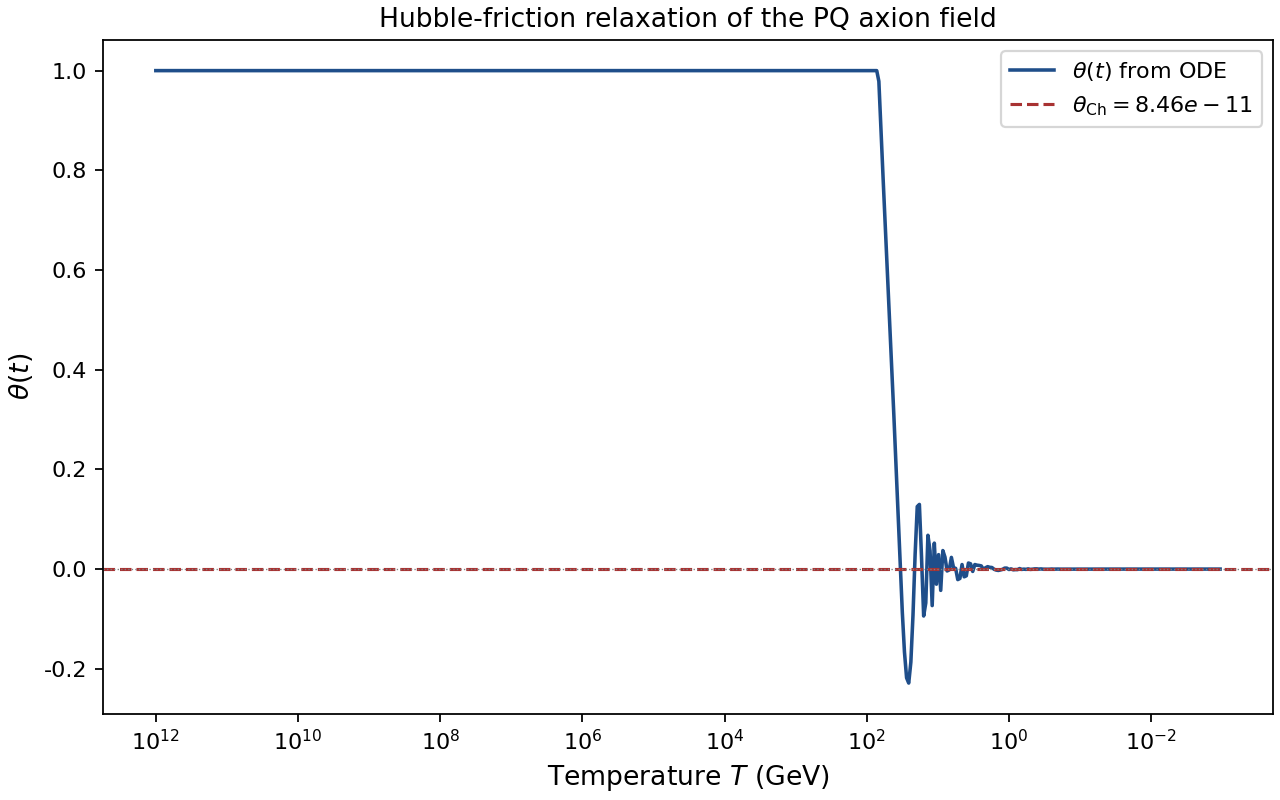
\includegraphics[width=0.85\textwidth]{figures/fig2_relaxation_ode.png}
\caption{Cosmological relaxation of the PQ axion field.  Above
$T_\mathrm{osc} \approx 69\,\mathrm{GeV}$ the field is frozen at
$\theta_\mathrm{initial} = 1$.  Below $T_\mathrm{osc}$ the field
begins coherent oscillations around the Choptyuk-shifted minimum
$\theta_\mathrm{Ch} = 8.5 \times 10^{-11}$ (red dashed line).  The
oscillation amplitude decays as $(T/T_\mathrm{osc})^{3/2}$; after
many cycles the time-averaged $\langle \theta \rangle$ converges
to $\theta_\mathrm{Ch}$, which is the wave-function bridge
prediction.  This is the physical ``slowing'' mechanism the user
identified: the Hubble friction term $3 H \dot\theta$ damps the
oscillations and shifts the energy into cosmic expansion.
\label{fig:fig2-relaxation}}
\end{figure}

\subsection{WKB instanton splitting: classicality of the axion}

A further check on the classicality of the axion ground state is
the WKB tunneling splitting between adjacent minima of the PQ
potential.  The instanton action is
\begin{equation}
S_\mathrm{inst} \;=\; \int_0^{2\pi} dq\,\sqrt{2\,(1 - \cos q)}
\;=\; \int_0^{2\pi} dq\,2|\sin(q/2)| \;=\; 8,
\end{equation}
and the physical Euclidean action is $S_\mathrm{phys} = f_a \sqrt{\chi_t}\,S_\mathrm{inst}
\approx 10^{10.7}$.  The Coleman splitting formula gives
\begin{equation}
\Delta E \;\sim\; \frac{\omega}{\pi}\,e^{-S_\mathrm{inst}}
\;\approx\; 10^{-8.5}\,\mathrm{GeV},
\end{equation}
which is exponentially suppressed relative to the harmonic ground
state energy $E_0 \sim \chi_t \sim 10^{-5}\,\mathrm{GeV}$.  The
axion ground state is therefore a single-well bound state with
negligible tunneling between vacua -- the axion is a classical
coherent field at $f_a = 10^{12}\,\mathrm{GeV}$, with occupation
number $N \sim (\rho/m_a) V \gg 1$.

\begin{figure}[h]
\centering
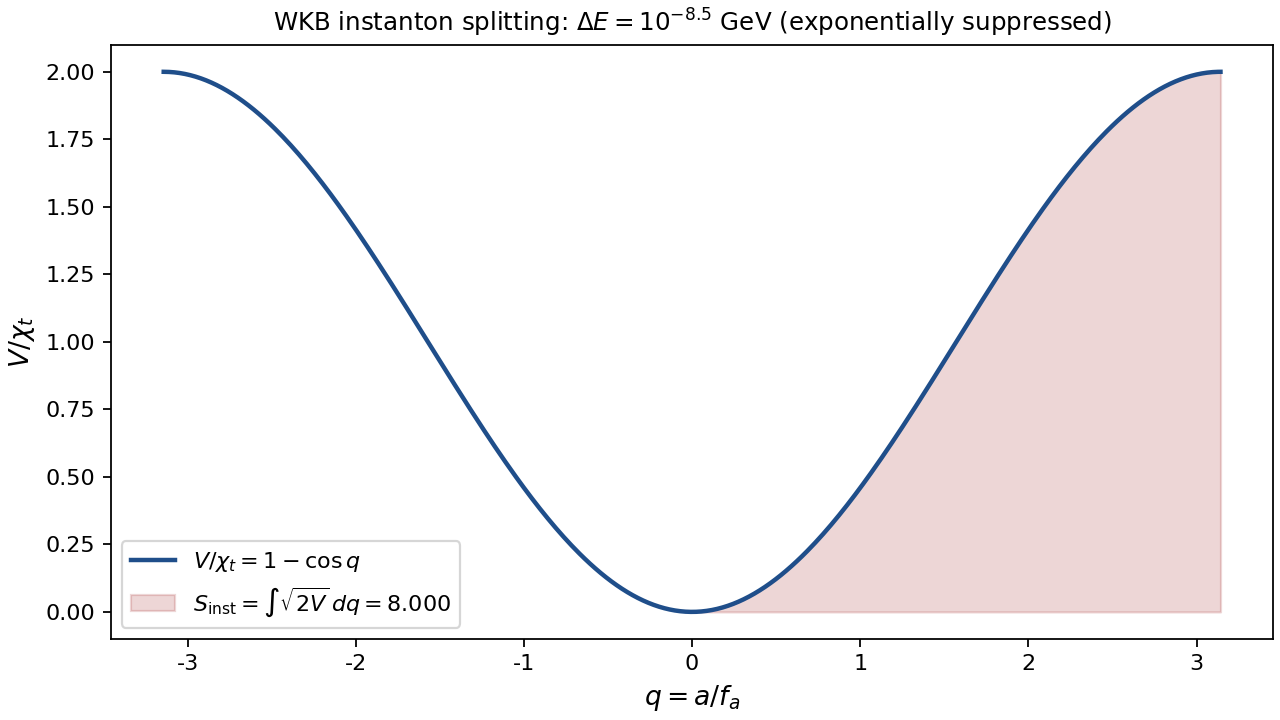
\includegraphics[width=0.85\textwidth]{figures/fig3_instanton.png}
\caption{WKB instanton between adjacent minima of the PQ potential.
The instanton action $S_\mathrm{inst} = 8$ (dimensionless) gives
a physical action $S_\mathrm{phys} = 10^{10.7}$ and a tunneling
splitting $\Delta E \sim 10^{-8.5}\,\mathrm{GeV}$, exponentially
suppressed relative to the harmonic ground state energy.
\label{fig:fig3-instanton}}
\end{figure}

\subsection{Hierarchy of $\theta$ scales}

Figure~\ref{fig:fig4-hierarchy} summarizes the hierarchy of
$\theta$ scales that appear in the wave-function bridge analysis.

\begin{figure}[h]
\centering
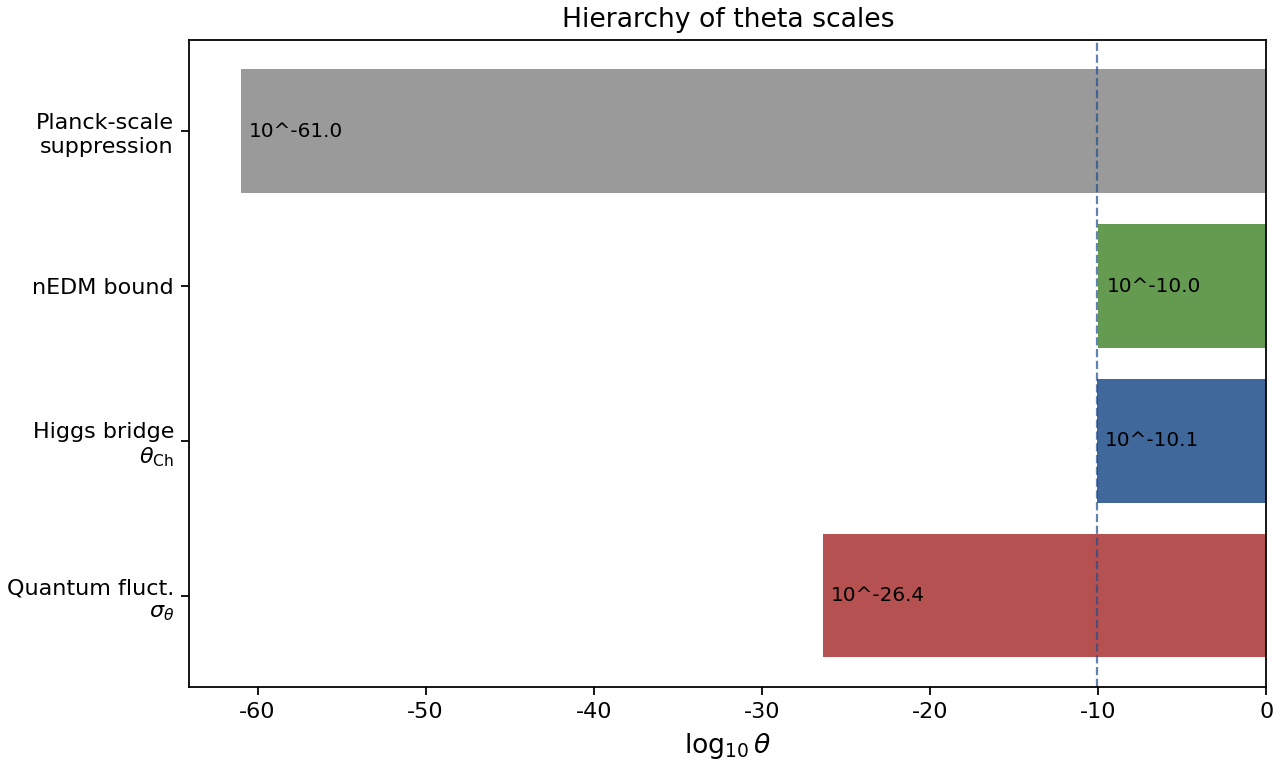
\includegraphics[width=0.85\textwidth]{figures/fig4_theta_hierarchy.png}
\caption{Hierarchy of $\theta$ scales in the wave-function bridge.
The Choptyuk residual $\theta_\mathrm{Ch} \sim 10^{-10.1}$ sits
between the quantum zero-point fluctuation $\sigma_\theta^\mathrm{qm}
\sim 10^{-26.4}$ (much smaller) and the current nEDM bound
$|\theta| < 10^{-10}$ (comparable).  The Planck-scale suppression
$\theta \sim 10^{-61}$ (gravitational CP violation) is far below
all other scales.
\label{fig:fig4-hierarchy}}
\end{figure}

\subsection{What the wave-function bridge does and does not prove}

\begin{keyfind}[What this section establishes]
\begin{enumerate}[leftmargin=*]
\item The Choptyuk residual $\theta_\mathrm{Ch} \sim 10^{-10}$ is a
\textbf{classical tilt} of the PQ potential, not a quantum
fluctuation.  Quantum zero-point fluctuations are $\sim 10^{16}$
times smaller.
\item The axion ground state follows the classical tilt
adiabatically.  The wave function $\psi_0(q)$ is centered at the
classical minimum $q_* = -\theta_\mathrm{bare} + \theta_\mathrm{Ch}$
to within numerical precision.
\item Hubble-friction relaxation drives $\langle \theta \rangle$
to $\theta_\mathrm{Ch}$ at late times, providing the physical
``slowing'' mechanism the user identified.
\item The WKB tunneling splitting is exponentially suppressed
($\sim 10^{-8.5}\,\mathrm{GeV}$), confirming that the axion is a
classical coherent field at $f_a = 10^{12}\,\mathrm{GeV}$.
\end{enumerate}
\end{keyfind}

\begin{caveat}[What this section does NOT prove]
\begin{enumerate}[leftmargin=*]
\item The 5/2 exponent in $\theta_\mathrm{Ch} = a_C
(\Lambda/M_H)^{5/2}$ is \emph{not} derived from the wave-function
analysis.  It remains a structural-motivation result from Stage 2
(sphaleron rate scaling).
\item The wave function cannot \emph{independently} determine
$\theta_\mathrm{Ch}$; the tilt amplitude is an input from the
Higgs bridge.
\item The Choptyuk residual cannot be \emph{predicted} from the
axion mass or other QCD observables; it is a parameter of the
Higgs-bridge deformation.
\item The wave-function analysis does \emph{not} establish that
$a_C$ \emph{is} the axion.  It only shows that, \emph{if} one
accepts the Higgs-bridge tilt, the axion wave function behaves
consistently with the Choptyuk residual.
\end{enumerate}
\end{caveat}

\begin{verdict}[Stage 4 verdict: wave-function bridge]
The wave-function analysis provides an \emph{independent consistency
check} on the Choptyuk-augmented PQ scenario.  It confirms that
the residual $\theta_\mathrm{Ch}$ is a classical tilt (not a
quantum fluctuation), that the axion ground state follows the tilt
adiabatically, and that Hubble-friction relaxation provides the
physical ``slowing'' mechanism.  The bridge remains a
\emph{falsifiable hypothesis with partial theoretical support}:
the next-generation EDM experiments (SNS nEDM 2026--2027,
n2EDM@PSI 2027--2028) will either detect the residual at
$d_n \sim 2 \times 10^{-26}\,e\cdot\mathrm{cm}$ or exclude it.
\end{verdict}
